% !TeX root = ../main.tex

\chapter{实验结果与分析}

\section{测量Casimir力曲线}
\subsection{用仪器自带的程序测量力曲线并与Lifshitz理论对比}
\paragraph*{}
我们首先使用的是仪器自带的程序测量Casimir力曲线。测量力曲线的具体步骤为:
\\1..根据上一章正式实验前的准备操作将小球进针至与金板接触的状态;
\\2.打开曲线测量窗口,在测量模式中选择"灵敏度",曲线类型中选择"力曲线";
\\3.设定适当的力-距离曲线测量参数:开始电压、结束电压和采集点数;
\\4.点击“开始测量”,获得力-距离曲线,如图\ref{fig:11}所示:
\begin{figure}
	\centering
	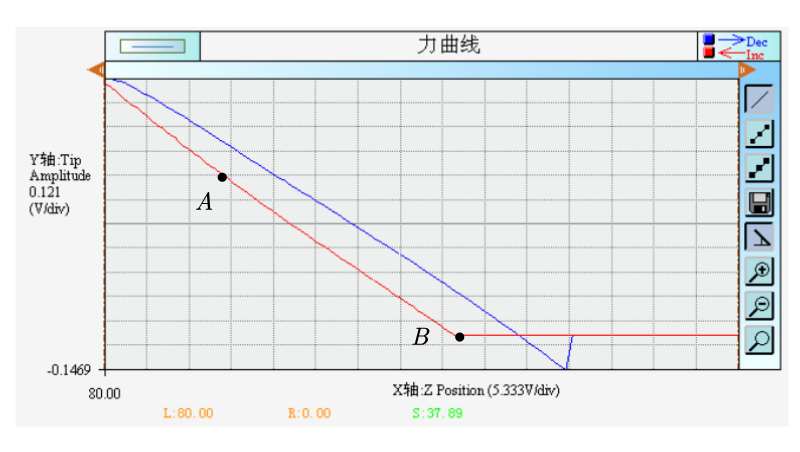
\includegraphics[width=0.7\linewidth]{figures/力曲线}
	\caption{力-距离曲线}
	\label{fig:11}
\end{figure}
\paragraph*{}
如上图所示,使用仪器自带的程序测量得到两条力曲线,红色的代表进针时的力曲线,蓝色的代表退针时的力曲线,由于退针时样品和针尖的接触面会形成化学键或存在其它粘附作用,针尖会粘附在样品表面一段距离,超过进针曲线中的初始接触点。当悬臂梁被提起一段高度后,针尖会脱离与样品的粘附,悬臂梁在样品表面上方重新恢复自由状态,可以根据退针曲线的跳变值测量出断裂键或粘附所需要力的大小。由于退针曲线存在四象限信号的突变,这会覆盖Casimir力的信号,我们只分析进针曲线。
\paragraph*{}
从力-距离曲线中,我们可以确定四象限的Up-Down信号与悬臂梁受力的关系。具体计算步骤如下:若悬臂梁的劲度系数$k$和压电陶瓷在z方向的伸缩系数$k_z$已知,假设小球与金板都是刚体,当它们处于接触的状态时,压电陶瓷在z方向的伸缩量就是悬臂梁的形变量。图\ref{fig:11}中A点对应的悬臂梁形变量和受力分别为:
$$
\Delta x=k_z\cdot(V_A-V_B)
$$
$$
F=k\cdot \Delta x= k\cdot k_z\cdot(V_A-V_B)
$$
\paragraph*{}
保存采集到的进针曲线数据,我们可以作图分析金球与金板之间距离非常近时的受力情况。图\ref{fig:12}内嵌的左图表示的是进针曲线,可以明显地看出当金球与金板距离很近时受到Casimir吸引力。取小球与金板之间的距离从0到500nm的一段重新作图,得到内嵌的右图所示的力曲线,图中黑色的曲线代表根据Lifshitz理论得出来的力曲线,蓝色的曲线代表实验测得的力曲线,可以看出实验和理论相符合。这里感谢张一驰同学编写的程序。
\begin{figure}
	\centering
	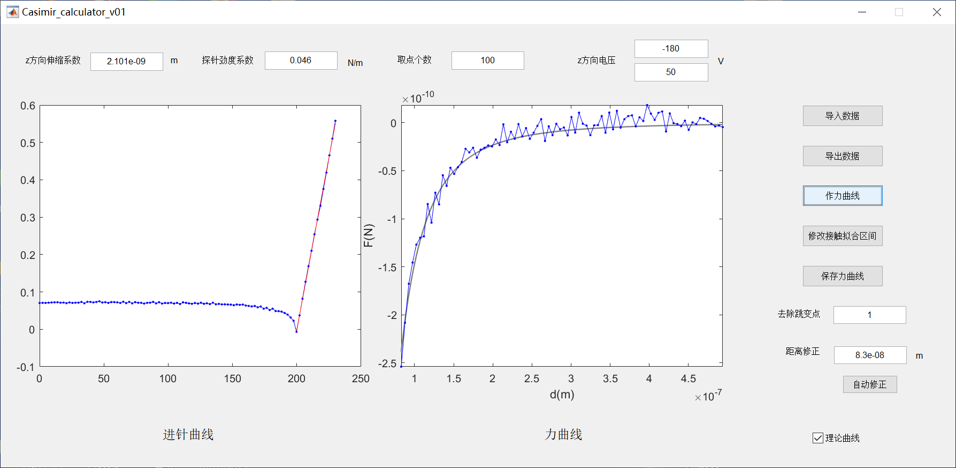
\includegraphics[scale=0.5]{figures/zyc力曲线}
	\caption{使用仪器自带程序测量得到的力曲线}
	\label{fig:12}
\end{figure}
\subsection{外接端口测量力曲线的方法介绍}
\paragraph*{}
我们扫描时必须实时地采集四象限的响应信号,而系统自带的软件无法实现这个功能,因此我们需要使用外接端口引出四象限的信号,并用计算机实时地采集引出的信号值。我们使用的是NI公司生产的“USB-6001”数据采集卡来采集信号,并编写了相应的采集信号的Labview程序。
\paragraph*{}
使用外接端口测量力曲线的具体步骤为:
\\1.打开曲线测量窗口,在测量模式中选择"灵敏度",曲线类型中选择"力曲线";设定适当的力-距离曲线测量参数:开始电压、结束电压和采集点数;
\\2.打开"Casimir信号采集程序.vi"软件,选择“信号采集器”功能模块,选择要存储的txt文件;
\\3.点击“开始测量”的同时点击"信号采集器"的开始按钮;
\\4.等到测量过程结束,点击"Casimir信号采集程序.vi"的停止按钮,停止采集四象限信号值。
\paragraph*{}
使用上述方法采集到的原始信号如图\ref{fig:13}(a)所示,横坐标表示加在压电陶瓷z方向上的电压,纵坐标代表采集到的四象限Up-Down信号值。由于进针结束时探针与样品处于接触的状态,最开始样品要先与探针分离,当样品下降到最低点后再逐渐开始升高,测量进针曲线,接着再测量退针曲线,在测量力曲线结束后继续升高样品,直到四象限的Up-Down信号值等于设定的参考值停止。去除曲线中的初始时刻样品与探针分离以及最后样品与探针接触上这两部分后得到如图\ref{fig:13}(b)所示的进针和退针曲线,再提取出进针曲线,如图\ref{fig:13}(c)所示,然后用类似图\ref{fig:12}的处理方法我们可以得出如图\ref{fig:13}(d)所示的力曲线,图中橙色的曲线代表Lifshitz理论模拟出的力曲线,蓝色的曲线代表实验测量得到的力曲线,可以看出实验数据和理论模拟相符。
\begin{figure}[h]
	\centering
	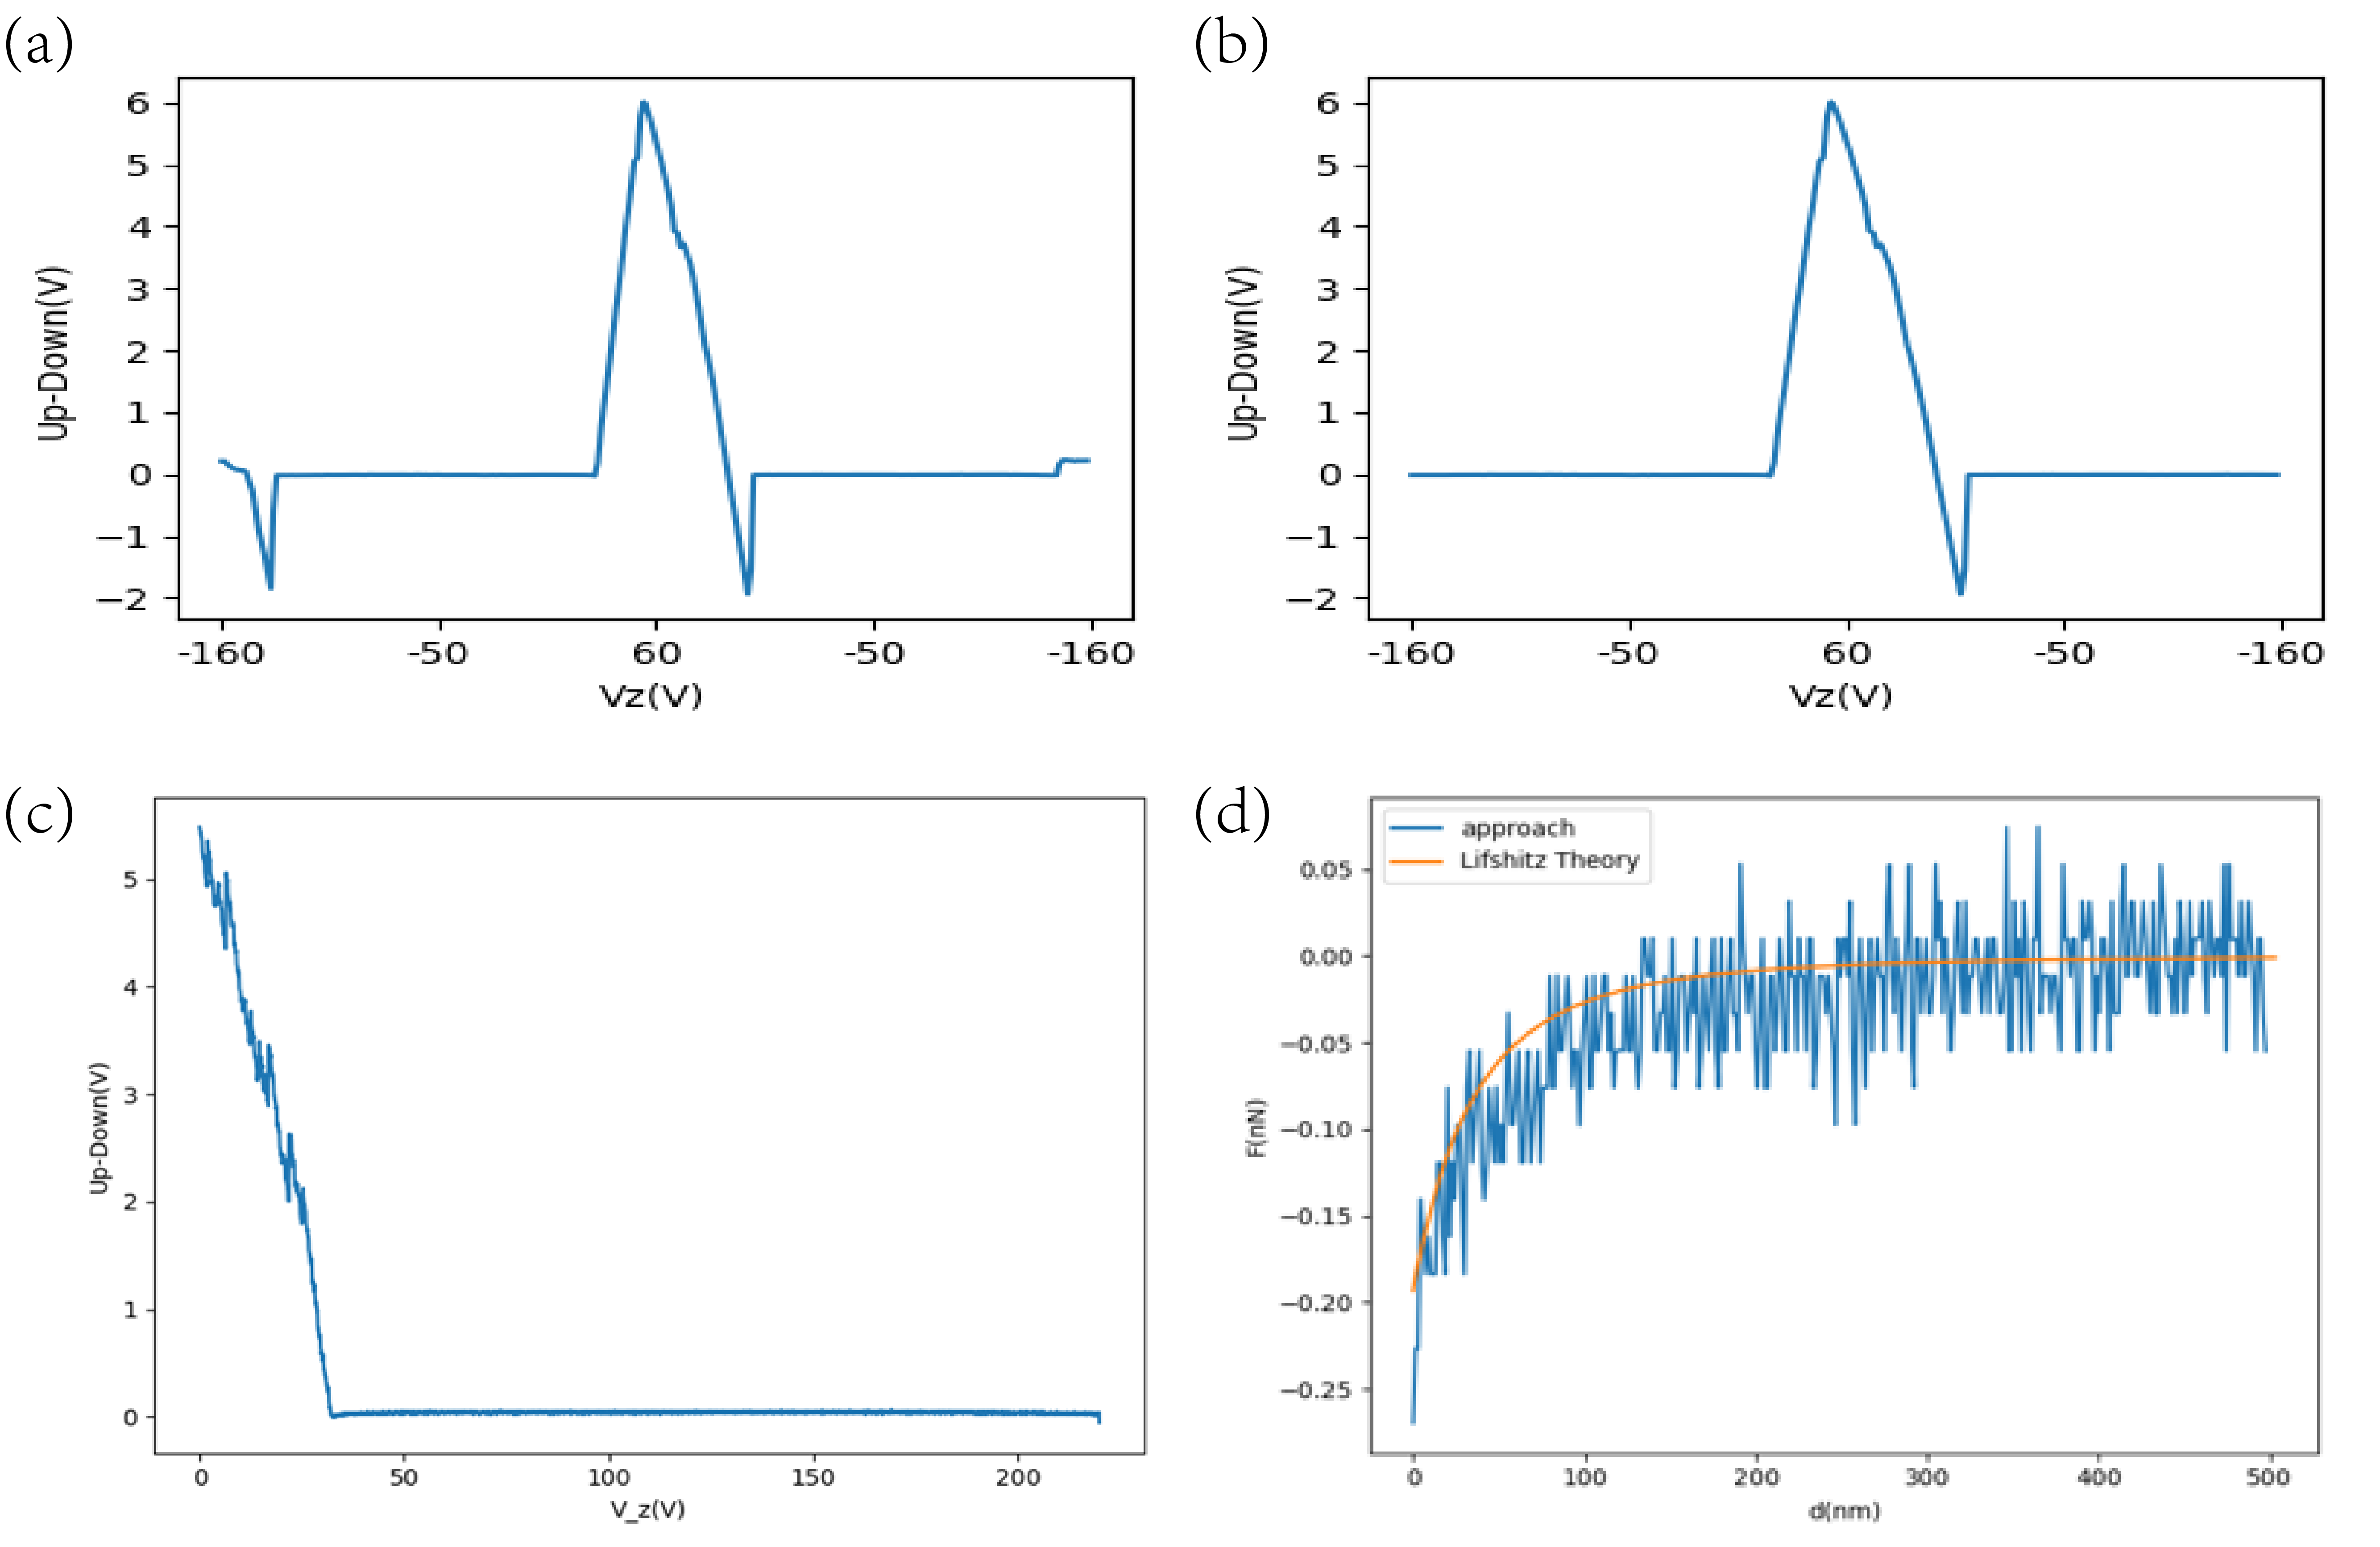
\includegraphics[scale=0.3]{figures/自测力曲线}
	\caption{外接端口测量力曲线(a)原始信号.(b)去除曲线中的初始时刻样品与探针分离以及最后样品与探针接触上这两部分后的信号.(c)进针曲线.(d)力曲线}
	\label{fig:13}
\end{figure}
\paragraph*{}
由于图\ref{fig:13}(a)(b)包含了很多我们不需要的信息,因此我编写了新的程序,用来方便的做出类似\ref{fig:13}(c)(d)的图并进行保存。改良后的数据处理步骤如下:
\\1.打开“Casimir信号处理程序.py”,并运行程序;
\\2.选择“力曲线”功能模块;
\\3.输入设置参数,包括:Vz的最大值,最小值,压电陶瓷z方向的伸缩系数,探针劲度系数,去除跳变点个数,距离修正以及选择是否显示理论曲线;
\\4.点击导入文件按钮,导入采集到的txt文件;
\\5.点击保存图像按钮,保存对应的进针曲线或者力曲线图。
\section{扫描样品}
测量得到Casimir力曲线后,接下来就是对样品进行恒高无接触式扫描,探索通过小球受到的Casimir力反应样品表面形貌变化的可能性。在扫描之前之前,有两点事项需要注意:1.样品的倾斜对于实验的影响。即使在扫描的方向上样品倾斜的斜率只有百分之一,由于我们扫描的范围大约为100微米,在这个范围内样品的高度仍然有1000纳米的起伏,因此,排除样品的倾斜情况对扫描的干扰是非常有必要的。测量样品的倾斜情况的方法如下:首先进针使探针和样品处于接触的状态,记录此时四象限Up-Down信号作为参考信号值,然后关闭仪器内部电路反馈,点击“单步进针”按钮使至屏幕上显示的$V_z$等于180V,使加在压电陶瓷上的电压完全取决于我们的外部输入电压.接着在压电陶瓷z方向上加上108V的电压,使样品向下运动约2微米,与针尖分离,然后沿着x方向加偏压,使样品向左移动一定距离,再缓慢减小加在压电陶瓷z方向上的电压,直到样品与探针接触,记录接触时加在压电陶瓷z方向的电压,换算成距离对应的就是在x方向上相距一定距离的两处高度差,将该高度差与水平移动的距离相除就能得到样品在x方向上的斜率。用同样的方法也可以得出样品在y方向上的斜率。这样在水平扫描过程中我们就可以修改程序,根据样品的倾斜情况实时地改变加在压电陶瓷z方向上的电压,以抵消样品的倾斜对于扫描的影响。2.压电陶瓷的畸变效应。如图\ref{fig:14}所示,扫描器伸缩的距离与所加的电压非线性关系;在电压增加的前段,扫描器伸长的距离慢于电压增加的后段;在电压减小的前段,扫描器缩短的距离快于电压减小的后段;畸变效应导致扫描器来回的路径不重合,扫描器伸缩的长度还与所加电压的过程有关,压电陶瓷的畸变效应会导致我们来回扫描探针接收到的力信号不重合,因此我们只选取采集单方向扫描的信号进行分析处理。
\begin{figure}[h]
	\centering
	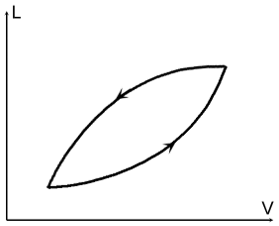
\includegraphics[scale=0.5]{figures/压电陶瓷的畸变效应}
	\caption{压电陶瓷的畸变效应}
	\label{fig:14}
\end{figure}
\subsection{一维的扫描}
\paragraph*{}
我们首先进行的是一维的扫描。扫描所用的样品为台阶高度约为80nm的金台阶样品,样品的刨面高度图\ref{fig:15}如图所示。
\begin{figure}[h]
	\centering
	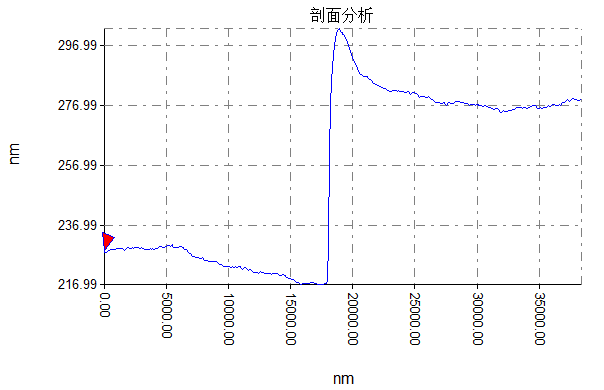
\includegraphics[scale=0.5]{figures/台阶刨面图}
	\caption{台阶样品刨面高度图}
	\label{fig:15}
\end{figure}
\paragraph*{}
扫描的信号采集与数据处理的具体操作为:
\\1..根据上一章正式实验前的准备操作将小球进针至与金板接触的状态;
\\2.点击"单步退针"按钮,直到$V_z$达到180V,再调节比例增益和积分增益为0,关闭回路的反馈,此时屏幕上的"Up-Down"值应该接近于0;
\\3.点击"单步进针"按钮,直到屏幕上的"Up-Down"值为2V左右;
\\4.打开”Casimir信号采集程序.vi”软件,选择“探测样品的倾斜情况”功能模块,点击上面的布尔开关使之处于打开的状态,设置Vx为8,点击运行程序按钮,观察左边Vz的波形图标,若Vz降到0V之前Up-Down均值一栏大于0.2,点击停止按钮,记录此时的Vz,然后再设置Vx为7,点击运行程序按钮,当Up-Down均值一栏大于0.2,点击停止按钮,记录此时的Vz,计算两次记录的Vz差值;若Vz降到0V之前Up-Down均值一栏一直小于0.2,设置Vx为-8,点击运行程序按钮,当Up-Down均值一栏大于0.2,点击停止按钮,记录此时的Vz,然后再设置Vx为-7,点击运行程序按钮,当Up-Down均值一栏大于0.2,点击停止按钮,记录此时的Vz,计算两次记录的Vz差值。再点暗右上方的布尔按钮,输入$\Delta X$=1,$\Delta Z$ =两次记录的Vz差值,点击运行,得到扫描过程中Z方向应加的电压信号波形公式(有时加在压电陶瓷上的电压会突变,造成斜率测量不准确,这种情况下需要我们先假设一个电压波形公式,并根据下一步测量的过程中逐渐修正公式,尽可能地消除样品倾斜对于实验的影响);
\\5.选择“确定扫描的偏移量”功能模块。在“Vz(x)”一栏输入上一步得到的公式,选择保存数据的txt文件,点击运行,直到"均值"一栏突变,停止运行程序,记录“Vz偏移量”;
\\6.选择“一维地扫描”功能模块。在“Vz(x)”一栏输入和上一步一样的公式,在“Vz偏移量”一栏中输入上一步得到的“Vz偏移量”稍大的值,选择保存数据的txt文件,点击运行按钮;
\\7.打开“Casimir信号处理程序.py”,并运行程序;
\\8.选择“绘制扫描图像”功能模块;
\\9.输入设置参数,包括:Vx的最大值,最小值,Vy的最大值,最小值,显示扫描的第几条曲线以及选择一维曲线按钮;
\\10.点击导入文件按钮,导入采集到的txt文件;
\\11.点击保存图像按钮,保存对应的一维扫描曲线。
\paragraph*{}
在控制样品与探针不同距离下一维扫描采集到的信号如图\ref{fig:16}所示。可以看出当探针距离样品很近时能够扫描到台阶信号,如图\ref{fig:16}(a)所示,但是由于噪声信号的干扰,不同高度扫描探测到的力信号之间没有明显的差别;当探针距离样品的距离大于40nm后,扫描到的台阶信号逐渐淹没在噪声信号之中,如图\ref{fig:16}(b)所示。
\begin{figure}[h]
	\centering
	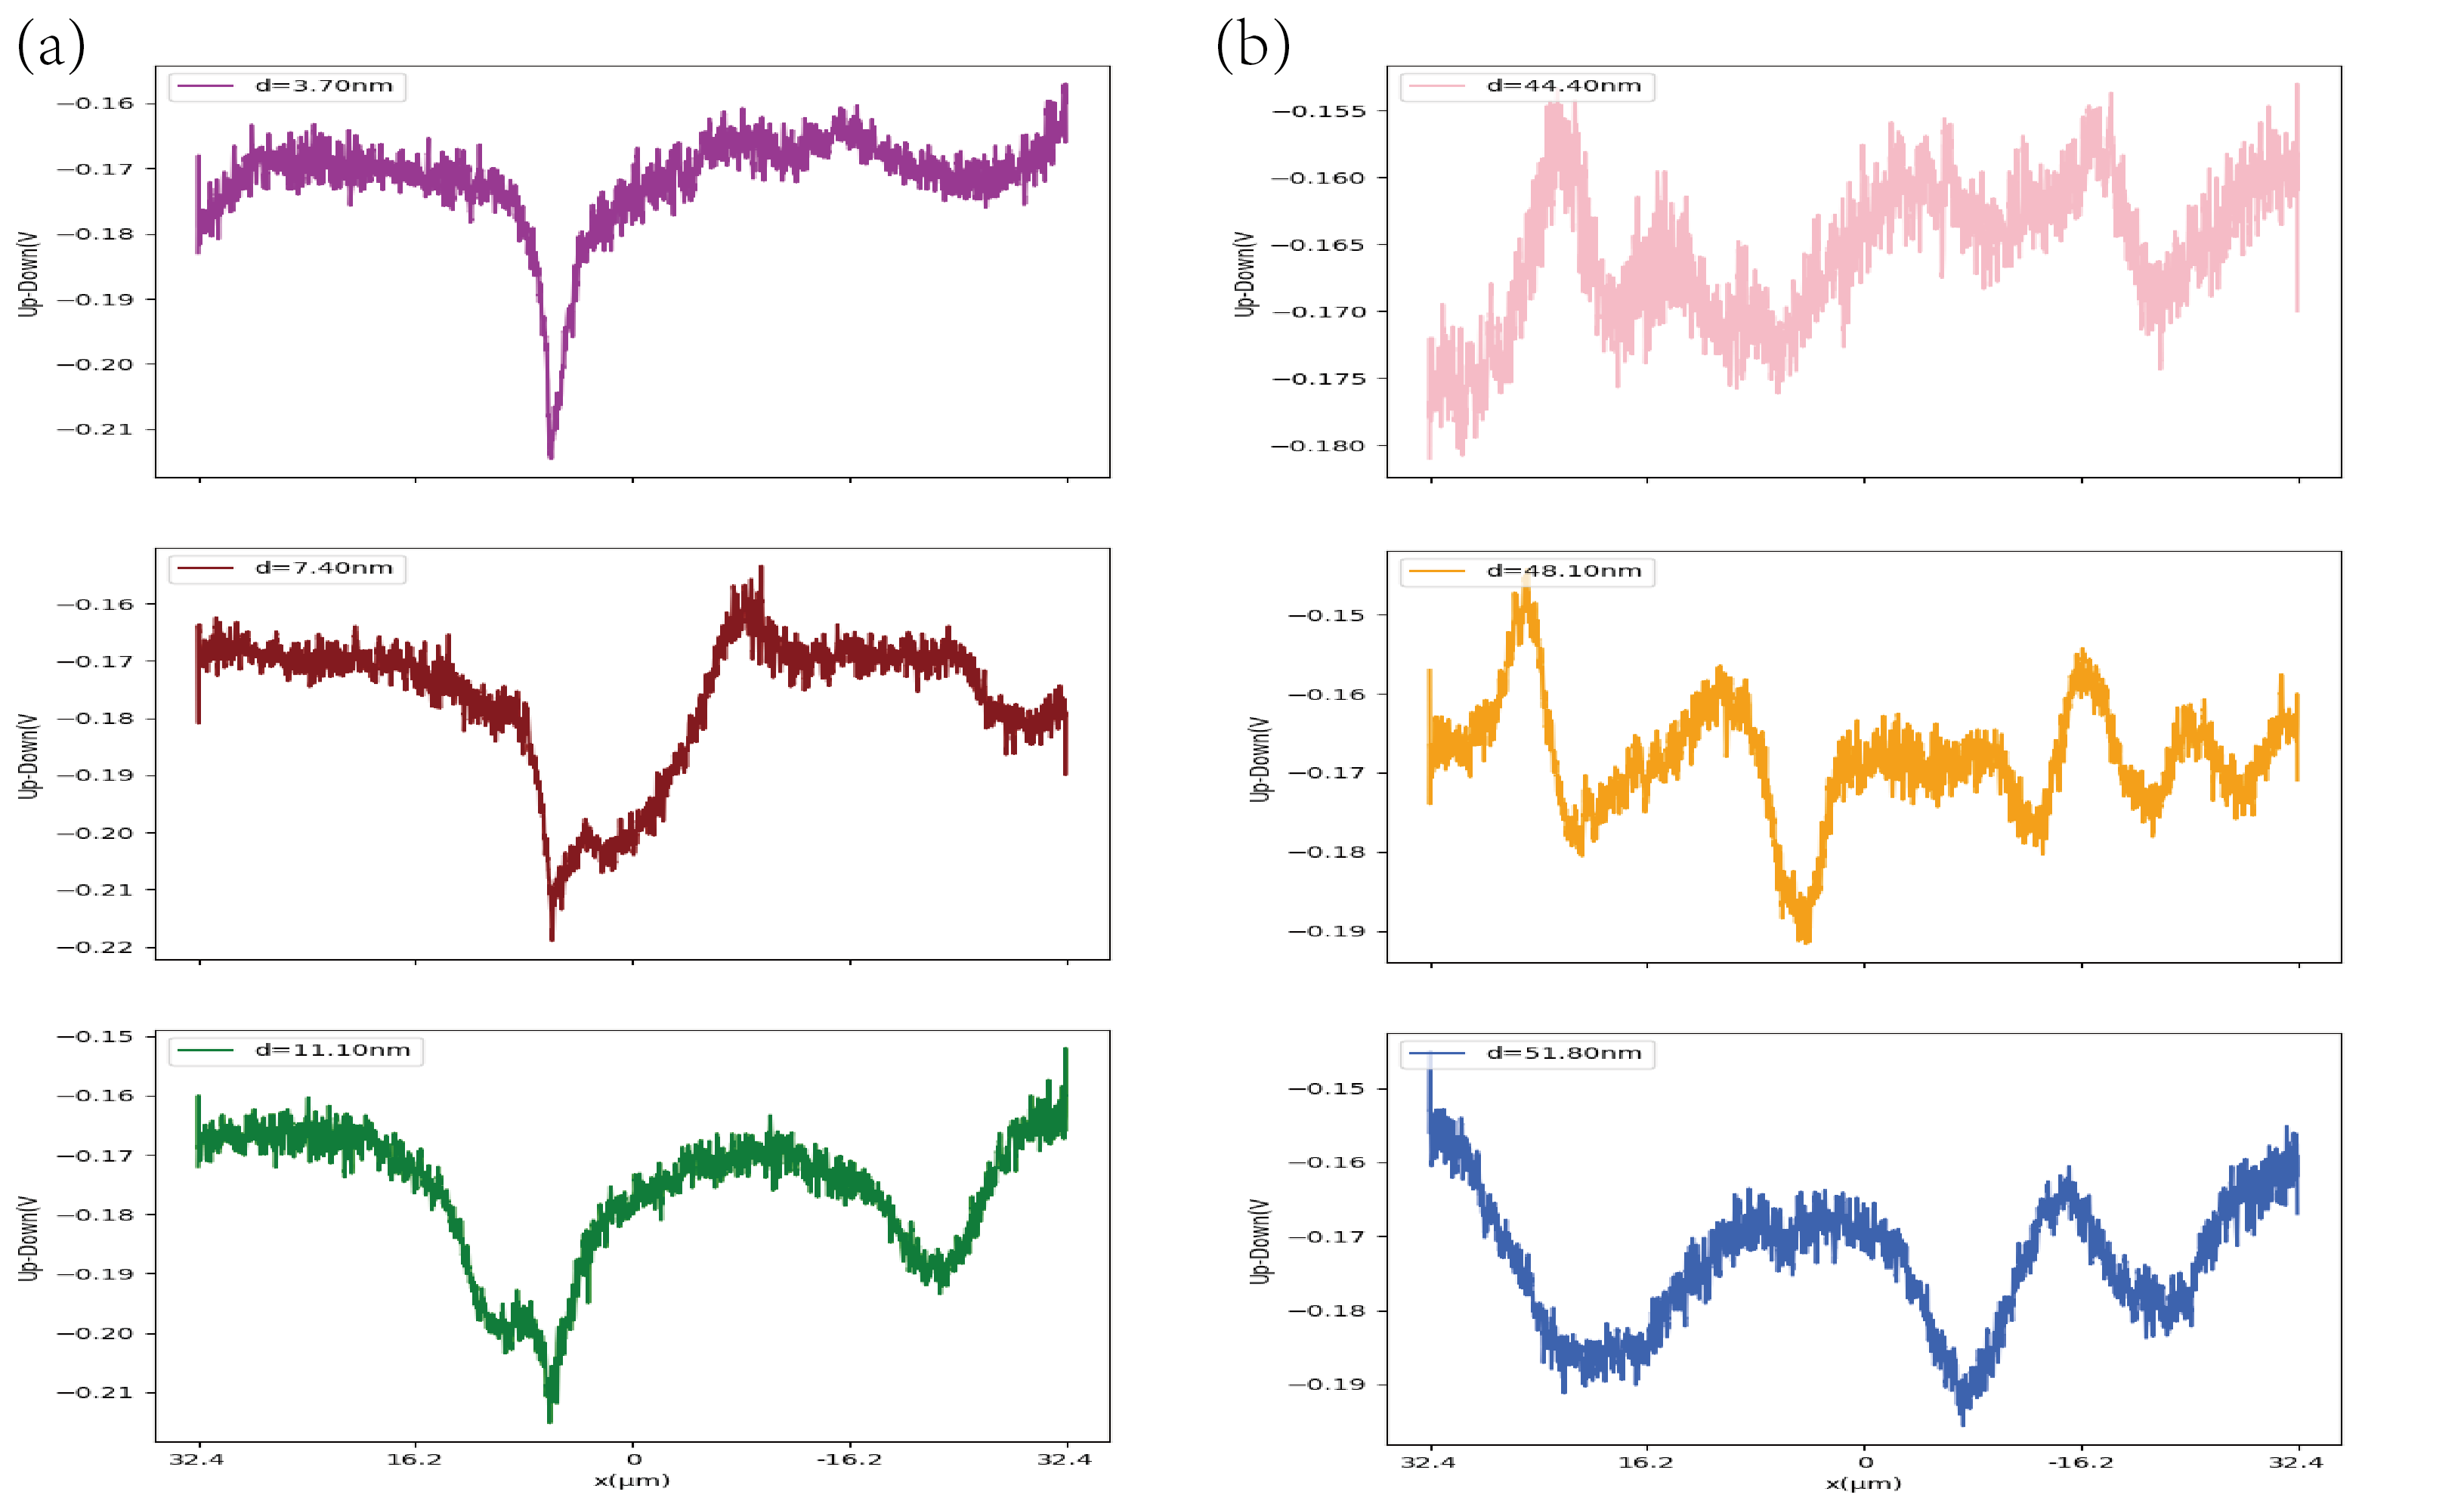
\includegraphics[width=15cm,height=11cm]{一维扫描.png}
	\caption{一维扫描采集到的信号(a)样品与探针间距小于15nm.(b)样品与探针间距大于40nm}
	\label{fig:16}
\end{figure}
\subsection{二维的扫描}
在一维的扫描的基础上每扫描一个周期,改变加在压电陶瓷y方向上的电压,以实现二维扫描。设定样品与探针之间的高度差为10nm左右,对金台阶样品扫描采集到的力信号如图\ref{fig:17}(a)所示。
\begin{figure}[h]
	\centering
	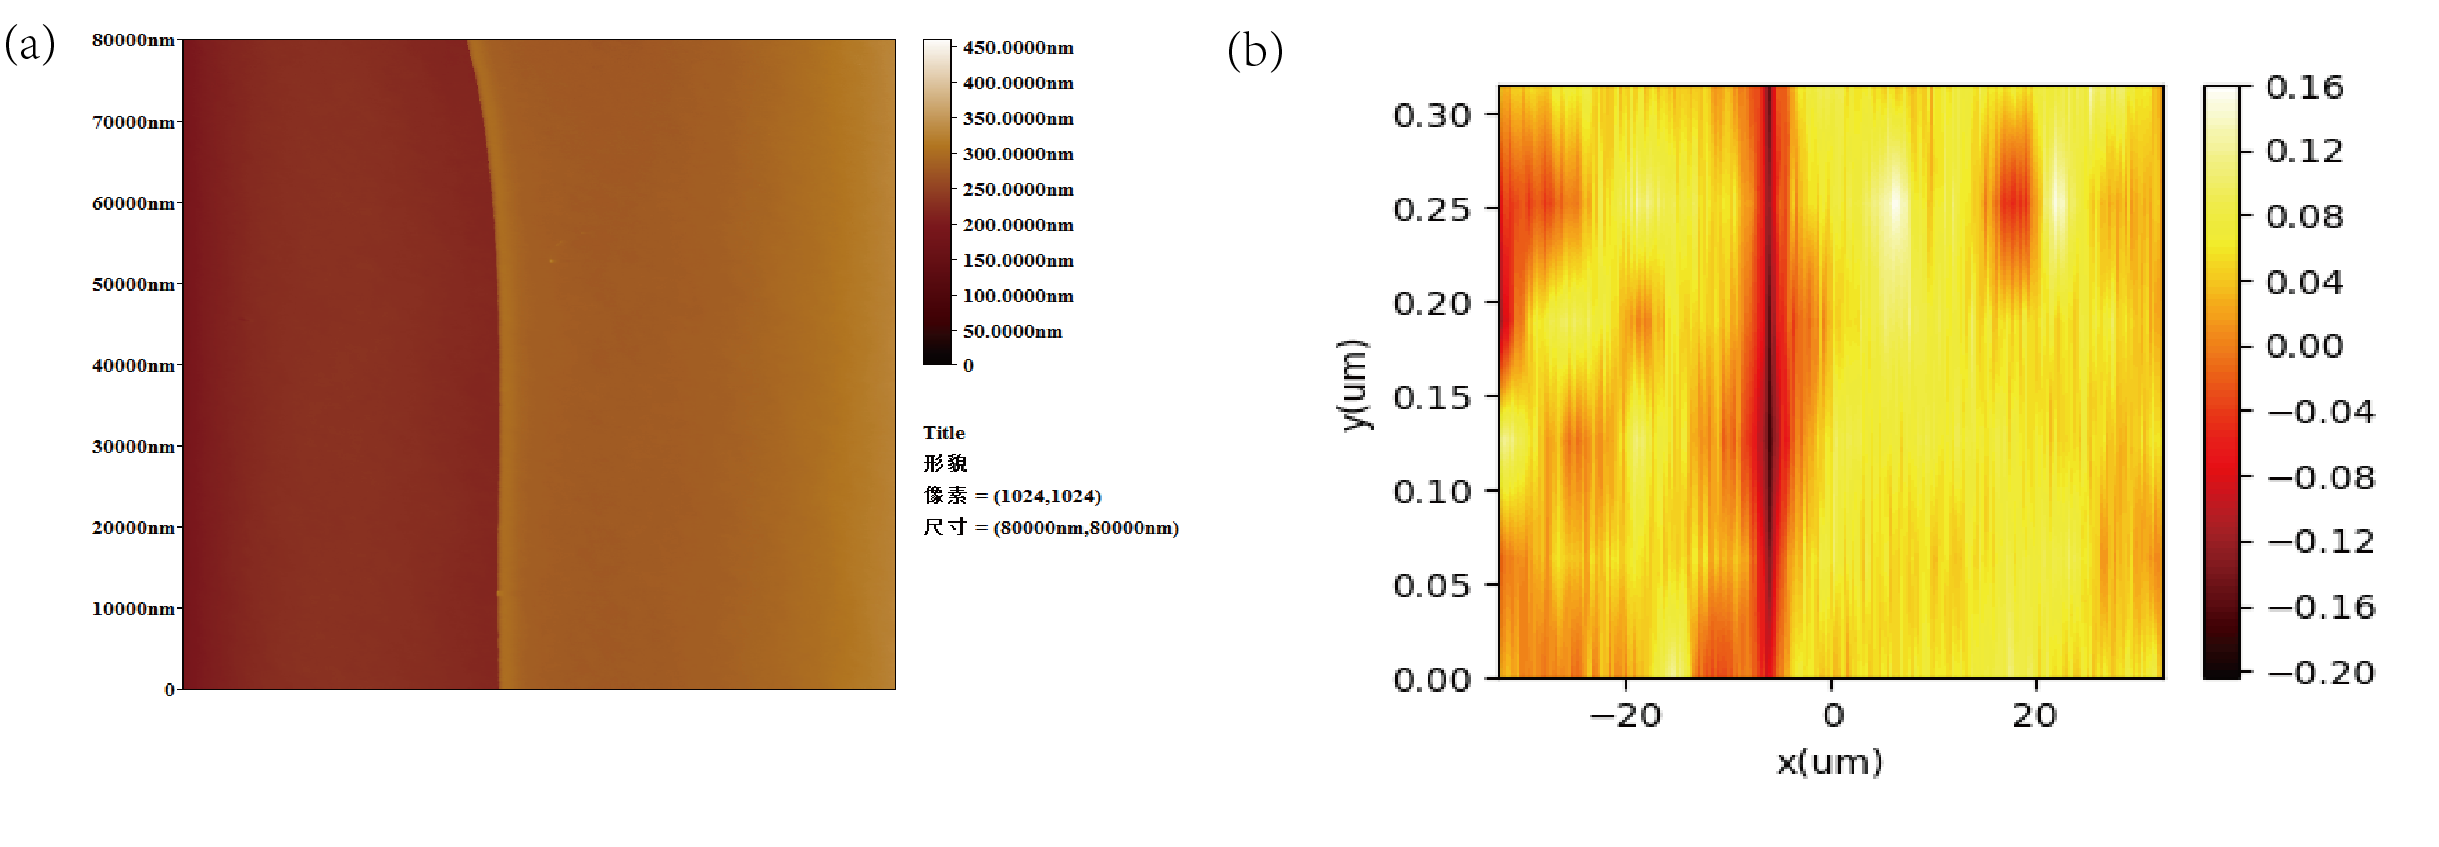
\includegraphics[width=15cm,height=6cm]{二维扫描.png}
	\caption{(a)使用AFM扫描得到的样品表面形貌图.(b)二维扫描采集到的力信号}
	\label{fig:17}
\end{figure}
\paragraph*{}
由图\ref{fig:17}可以看出二维扫描可以探测出台阶的存在,但是如何减小噪声信号的干扰,仍然是需要考虑的问题。